\begin{figure*}[!t]
\centerline{\includegraphics[width=0.88\textwidth,page=2]{../figures/main_figures_draft.pdf}}
\caption{\textbf{Thermodynamic sources.} (\textbf{A}) Provenance of the
protonation model. Every ladder behind the shipped energies comes from one
ChemAxon Marvin~26.1 regeneration; the open predictions ship alongside but are
not mixed into the energies. (\textbf{B}) Reactions carrying a real energy from
each source, no-estimate placeholders excluded. (\textbf{C}) Reported
uncertainty, on separate axes because the three differ by more than an order of
magnitude; a common axis would compress two of them to a spike.}
\label{fig:thermo}
\end{figure*}

\subsection{Thermodynamics}\label{sec:results-thermo}

%% Counts measured 2026-09-08 from Biochemistry/reaction_*.json after the
%% Marvin 26.1 rebuild. Placeholders excluded per source: group contribution
%% dg = 1e7 (26,555 records); eQuilibrator sigma >= 2500 kcal/mol (3,386),
%% which is that source's refusal marker rather than an error bar.
The three predictors cover comparable fractions of the database and disagree
substantially about how well they do it (Figure~\ref{fig:thermo}B). Group
contribution stores a value for essentially every reaction, but 26,555 of those
are a no-estimate placeholder; excluding them it covers 29,447 reactions,
against dGPredictor's 29,617 and eQuilibrator's 21,789. Coverage counts drawn
from raw entry counts overstate group contribution by a factor of two, and
eQuilibrator by 3,386 --- the reactions it declines to decompose, which it
marks with a refusal-scale uncertainty rather than an absent record.

Uncertainty is reported on scales differing by more than an order of magnitude
(Figure~\ref{fig:thermo}C): median 0.63\,kcal\,mol$^{-1}$ for eQuilibrator
against 10.41 and 17.01. A consumer choosing by smallest reported error would
systematically choose the source that understates it, which is the argument
against promoting any single source.

Protonation provenance is uniform in tool but not in vintage
(Figure~\ref{fig:thermo}A). Of 28,992 compounds, 19,657 (67.8\%) carry a ladder
from this release's Marvin~26.1 run, 4,351 (15.0\%) retain ChemAxon ladders
carried over from the pinned eQuilibrator release, and 4,984 (17.2\%) resolve to
none. The two denominators disagree sharply, as they did for the layered
scheme this replaces: only 6.1\% of the 25,175 scored reactions are resolved wholly by the
new run, because the carried-over minority are the cofactors that appear
almost everywhere, and 93.4\% of reactions touch at least one of them. A
regeneration can reach most compounds and still leave most reaction traffic
standing on inherited values.

\paragraph{A caveat on the rebuild.} Moving to a single protonation model
shifted 129 reactions by more than 10\,kcal\,mol$^{-1}$ relative to the previous
release --- largely glycans and other large polyanions whose partners were
re-protonated on a different basis, so a site on one side is no longer cancelled
by the same site on the other. They ship with a low-confidence flag
(Supplementary Table~S2). The mechanism is the transition between models rather
than an inconsistency inside this build. Neither the flagged value nor the
previous release's can be checked against measurement: none has an experimental
match, and in several cases the previous agreement came from two errors
cancelling.
